\cleardoublepage\chapter{Introduction}
\minitoc\label{sec:introduction}\vspace{.5cm}

\section{Background and Motivation}
A physical tunnel allows vehicles to move between 2 places indepently from surrounding geography. 
Similarly, network tunneling is a mean to organize traffic between host A and B in a way that:

\begin{itemize}
    \item Abstracts the underlying path over the public network: Applications binding to the tunnel are not aware of the real paths that packets take.
    \item Encapsulates and encrypts: Middle man - even can intercept the traffic - can't always determine if a network frame belongs to the tunnel or a tunnel is being used, nor decrypt the content.
\end{itemize}

A \ac{VPN} is a application build on top of a tunnel to connect 2 networks, effectively allow its host to access the other internal network remotely.
Well known \ac{VPN} applications can be named: \ac{wgpage}, \ac{ovpnpage}, IPsec, PPTP, PPPoE, L2TP, ...
Although different in level of operation (Network layer, Data Link layer) and operation space (kernel or user space), they generally share the same concept of single link: the tunnel utilizes one single network link to transmit and receive the tunnel packets. 
The other concept, namely \textit{multipath}, would deploy multiple network links so it can achieve higher reliability through redundancy or higher bandwidth through combining links, even though these characteristics are more relevant to environment such as infrastructure, datacenter or industrial application rather than end-user usage.
There are protocols such as \ac{MPTCP}, \ac{SCTP} that implement the concept, albeit in form of non-sharable connection.
A non-share connection is initiated similarly to initiating a socket and can only be used by the caller program. 
This severly limits the capability to control, schedule and share multipath resources between multiple applications in an effective manner, i.e prioritizing, buffering ... 
These require centralized orchestration level of control over all communication channels by a control plane, which doesn't exist for these protocols.

We propose another tunnel implementation: \ac{MTX}. 
The tunnel will have multipath support by design, allow multiple applications to share the connection simultainously, and be built based on Linux's \ac{xdppage} socket family.
Using the latest native Linux's technology, the implementation is expected to performance-wise outperform any userspace implementation while retain compatibility with existing systems and code base's simplicity. 
Support for multiple connection links offers reliability, large raw-bandwidth and a rich set of configuration to appications binding to the tunnel, makes it suitable for high demand use-cases such as industry, data center, telecommunication hub. 
In this document, an enhancement for the 5G's GTP-U protocol with \ac{MTX} library will be investigated. GTP-U is the protocol that helps UPF and gNodeB functions of a 5G system communicating, which demands both bandwidth and stability and therefore is a suitable match for a \ac{MTX} demostration.


\section{Problem Statement}\index{Requirements}
% In this section, the problems with single-link tunnel will be presented.
% Combine links
The most commonly used technologies for communication in datacenter and \ac{HPC} environment are Ethernet and \ac{infinibandpage} (\Cref{fig:introduction:Interconnect_Technologies_500_supercomp}), which currently offer 100-200Gb/s bandwidth per line \cite{ethernet_roadmap}\cite{infiniband_roadmap}.
These kind of bandwidth between computers (or inter-system) are nontheless impressive, yet not comparable to the system's internal connection, i.e inter-chiplet bridge \textit{Infinity Fabric} used in AMD's Zeppelin SoC provides 256GB/s in-package bandwidth \cite{burd_zeppelin_2019}, and up to 800GB/s connection in GPUs peer-to-peer test \cite{amd_infinity_architecture}.
This means even when invested in the current latest networking hardware, the connection between computer instances might be the bottleneck for certain applications that require distributed computation, for example large \ac{AI} or simulation model.
In this case, a multipath tunnel can hide hide the multipath details of merging multiple links from the applications, effectively scales up the network capacity horizontally.
The tunnel thus allow datacenter usage benifits from having larger combined bandwidth using current technology, but also is a neccessary tool to overcome eventual physical and economical limitation in the future.
For less demanding usages, aggregation is an affordable method to build fast connection from available hardware \todo{improve}.

% Reliability
Connection's reliability is closely related to the failure probabilities of the individual links and nodes (component reliability, can directly effect service availability) \cite{shooman_algorithms_1995} and the \ac{QoS} parameters \cite{gozdecki_quality_2003}.
Common connection's \ac{QoS}  parameters can be named: latency, peak throughput, jitter.
Depends on the use case, reliability of the connection can be a \ac{QoS} measurement factor (i.e commercial network provider) or a strict requirement (i.e critical application).
Generally, 2 non-exclusive stratergies are often used to increase a connection's reliability: through fortifying individual link, or redundancy.
A connection's failure probability can be reduced by upgrading to a more resilent but expensive link or equipping with multiple failover lines. 
Similarly, while better hardware can eliminate many \ac{QoS} inadequacy problems, having multiple links (or routes) each optimized for a type of appliance is certainly more suitable and affordable for the operator, especially if the data traffic is heterogeneous \cite{chen_overview_1998}.
A multipath tunnel with flow-aware capability can be used in this case to manage the underlying links as an abstraction layer for the applications that utilize the connection. \todo{improve} \todo{more about QoS}

%  heterogeneous data traffic

%%
% Combine with a powerful CPU, networking application based on technologies such as \ac{dpdkpage} can saturate even a 100Gbit line using a single CPU core \cite{intel_dpdk_perf}. 
% However, this can be improved by combining bandwidth of many links. 
% A multipath tunnel will create a logical NIC for application, effectively abstracts the management, orchesteration tasks for the applications.
% \todo{sota: how these are being done in real life?}
% Such method can be useful for long term and short term usage: using existing technology and hardware to achieve higher bandwidth to reduce cost, and overcome physical limitation.

\begin{figure}[H]
	\centering
	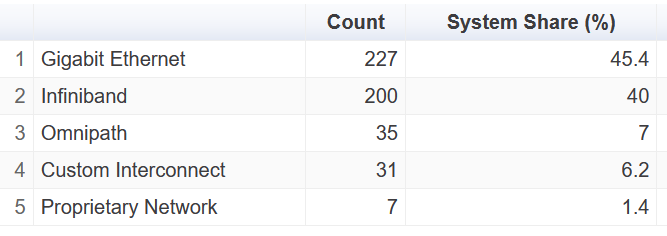
\includegraphics[width=0.8\textwidth]{resources/images/Interconnect_Technologies_500_supercomp.PNG}
	\caption{Interconnect technologies of top 500 super computers, 2023 edition as tracked by TOP500 project \cite{Interconnect_Technologies_500_supercomp}}
    \label{fig:introduction:Interconnect_Technologies_500_supercomp}
\end{figure}

\todo{other: latency, ...}

% Perf: userspace vs kernelspace process
% Omitting trivial tasks such as authentication and handshake, tunneling operation including the following steps: acquiration of ingress data stream (send to tunnel by application), process of ingress data (convert data into stream of tunnel packets, often through encapsulating with tunnel header, encrypting, compressing), and reverse on the receiving end (extrating original data from tunnel packets and delivering to application) \todo{cite+improve}.
% Apart from scaling the underlying system vertically (i.e by using more powerful hardware) or using a lower-level programing language, the most significant factor that could affect the performance of a single-link tunnel implementation is how ingress data is handled.


% \sidenote{State of the Art}
% \todomid{write about the State of the Art}

% \sidenote{Issue:\\Example 1}
% \todomid{write about the first issue}

% \sidenote{Issue:\\Example 2}
% \todomid{write about the second issue}

% \sidenote{Synopsis}
% \todomid{write about the synopsis of the issues and \Cref{fig:intro:c}}

% \begin{figure}[htbp]
%     \centering
%     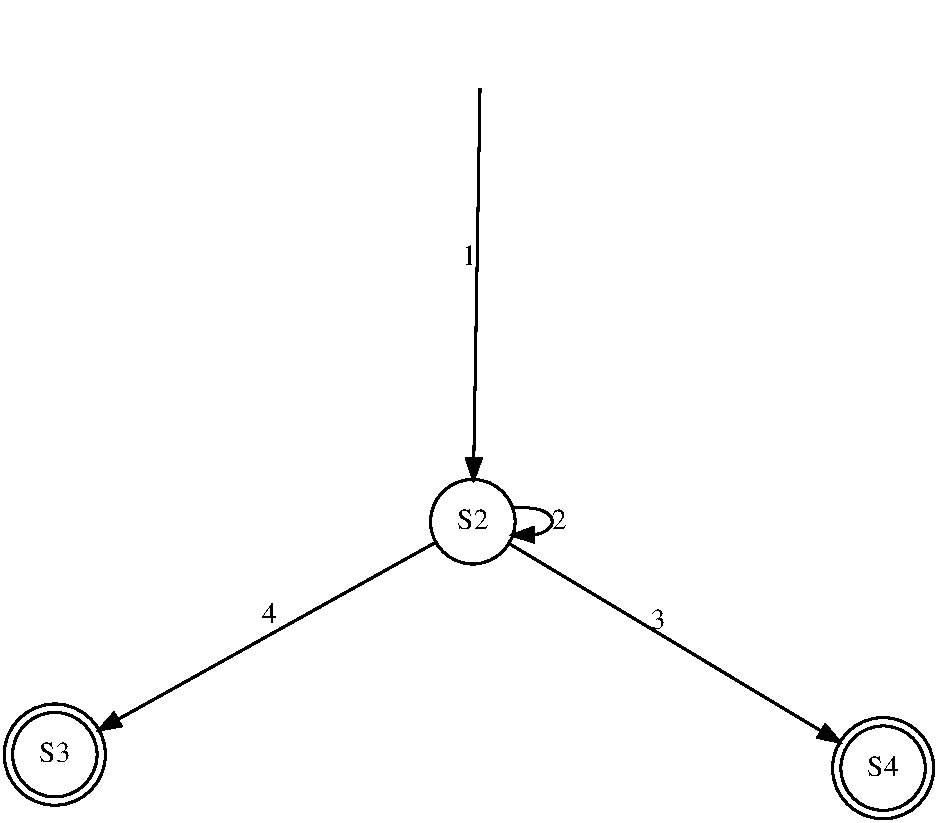
\includegraphics[width=.5\textwidth]{resources/images/job_lifecycle}
%     \caption{Relationship between issues}\label{fig:intro:c}
% \end{figure}

\section{Assumptions and Scope}

% \sidenote{Research Assumptions}
% \todomid{write about the research assumptions~\cite{li2002design}}
Besides the reliability's \ac{QoS} chracteristic, we define the metrices to measure performance of a tunnel as follow:
\begin{itemize}
    \item Bandwidth: Quantity of data that can be transmitted through per second, usually measured in Mega Bit per Second (Mb/s) or Giga Bit per Second (Gb/s)
    \item Latency: Delay, measured in microsecond (usec) or millisecond (ms). Latency introduced by the tunneling process at both ends compared to sending data over the same public path without the tunnel.
    \item System load: Tunneling process costs CPU time and RAM usage.
\end{itemize}

The project is inspired by \ac{5G}'s \ac{NFV} and \ac{SDN} influenced specification.
Being regconized as the 2 technology enabler for realizing 5G networks, they allow concepts such as \textit{Slicing}, hardware-software and control-data plane decoupling \cite{yousaf_nfv_sdn_key_techno_for_5g2017} \cite{open_baton} which make \ac{5G} network a much more capable network standard than its predecessor while remains flexible and agile for operators.

\todo{5G related to cloud-native. Mutipath -> upstream need bigger and reliable lines}

% \sidenote{Research Scope}
% \todomid{write about the research scope --- \Cref{fig:intro:a,fig:intro:b,fig:intro:c}}


\section{Objectives and Contributions}

% \begin{figure}[htbp]
%     \centering
%     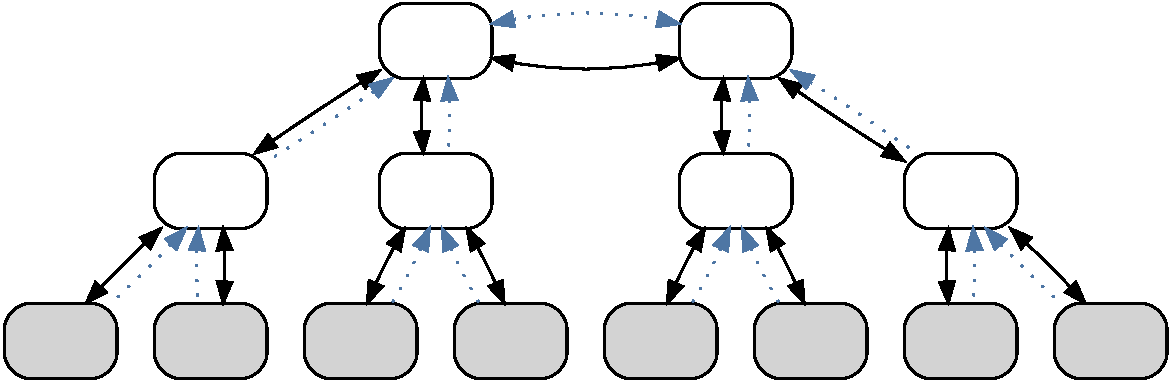
\includegraphics[width=.55\textwidth]{resources/images/example3}
%     \caption{Structure of research}\label{fig:intro:struct}
% \end{figure}

% \sidenote{Research Objectives \& Contributions}
% \todomid{write about the research objectives and \ac{DBpedia} and \Cref{fig:intro:struct}}

% \section{Methodology and Outline}

% \todomid{write about the research outline and \Cref{fig:intro:methodology}. Summarize \Cref{sec:introduction,sec:sota,sec:reqs,sec:contrib1,sec:contrib2,sec:contrib3,sec:eval,sec:summary}.}

% \begin{sidewaysfigure}
%     \centering
%     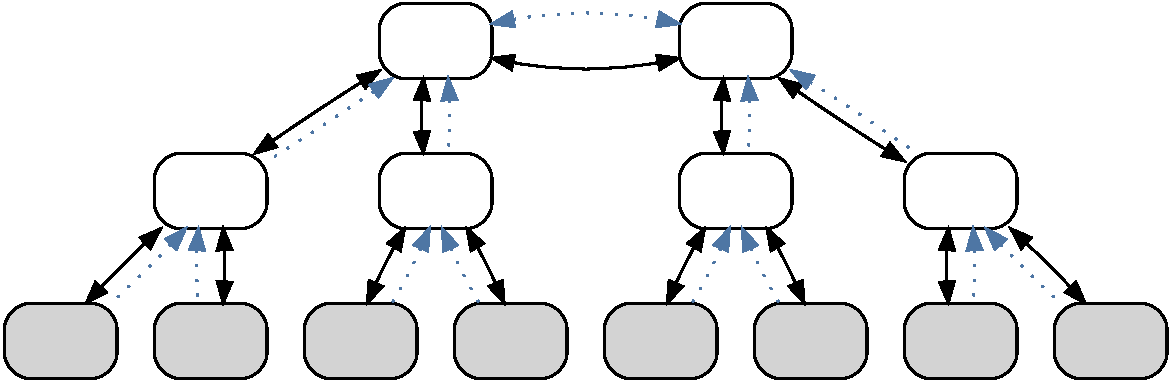
\includegraphics[width=.7\textwidth]{resources/images/example3}
%     \caption{Workflow of the research and structure of the thesis}\label{fig:intro:methodology}
% \end{sidewaysfigure}
